\documentclass{article}
\usepackage{../acad} % https://github.com/rstanuwijaya/latex-template

\renewcommand{\sectionPrefix}{}
\usepackage{listings}
\usepackage{xcolor}
\usepackage[]{minted}

\definecolor{codegreen}{rgb}{0,0.6,0}
\definecolor{codegray}{rgb}{0.5,0.5,0.5}
\definecolor{codepurple}{rgb}{0.58,0,0.82}
\definecolor{backcolour}{rgb}{0.95,0.95,0.92}

\lstdefinestyle{mystyle}{
    backgroundcolor=\color{backcolour},   
    commentstyle=\color{codegreen},
    keywordstyle=\color{magenta},
    numberstyle=\tiny\color{codegray},
    stringstyle=\color{codepurple},
    basicstyle=\ttfamily\footnotesize,
    breakatwhitespace=false,         
    breaklines=true,                 
    captionpos=b,                    
    keepspaces=true,                 
    numbers=left,                    
    numbersep=5pt,                  
    showspaces=false,                
    showstringspaces=false,
    showtabs=false,                  
    tabsize=2
}
\lstset{style=mystyle}

\title{PHYS 5120 HW1}
\author{TANUWIJAYA, Randy Stefan \footnote{\LaTeX\ source code: \url{https://github.com/rstanuwijaya/hkust-computational-material/}}\\ (20582731) \\ rstanuwijaya@connect.ust.hk}
\affil{Department of Physics - HKUST}
\date{\today}

\begin{document}
\maketitle
\begin{section}{The linear and nonlinear pendulums}
Consider a pendulum with a arm of length $l = \SI{10}{cm}$ holding a bob of mass $m$. The arm is massless. The gravitational acceleration $g = \SI{9.81}{m/s^2}$
\begin{enumerate}[1.]
	\item A simple pendulum is linear, i.e., $\sin{\theta} \approx \theta$. Write an equation of motion for the pendulum using Newton's second law. Derive the analytic solution. How long is the swing period?

	\begin{tcolorbox}
		The force acting on the pendulum along and perpendicular to the arm are given by:

		\begin{align}
			\Sigma F_{\parallel} & = T - m g \cos{\theta} = 0               \\
			\Sigma F_{\perp}     & = - m g \sin{\theta} = m r \ddot{\theta}
		\end{align}

		For small $\theta$, $\sin{\theta} \approx \theta$, we can solve the ODE by assuming $\theta = \theta_0 e^{i \omega t}$ and $\ddot{\theta} = - \omega^2 e^{i \omega t}$. Thus,

		\begin{align*}
			- m g \theta                  & = m r \ddot{\theta}                                                \\
			- m g \theta_0 e^{i \omega t} & = - m r  \omega^2 e^{i \omega t}  \iff \omega = \sqrt{\frac{g}{l}}
		\end{align*}

		Therefore,
		\begin{equation}
			\boxed{
				T = \frac{2\pi}{\omega} = 2\pi \sqrt{\frac{l}{g}} = \SI{0.634}{s}
			}
		\end{equation}
	\end{tcolorbox}

	\newpage
	\item The pendulum is released from a standstill at $\theta=2.4^\circ$. Write a program to solve the linear pendulum using the velocity Verlet method and a	proper time step.

	\begin{tcolorbox}[breakable]
		The follwing code plots the comparison between the analytical and numerical solutions.


		The analytical solution to the angle of the linear pendulum is given by:
		\begin{equation}
			\theta(t) = \theta_0 \cos{\left( \sqrt{\frac{g}{l}} t \right)}
		\end{equation}

		Whereas for the numerical solution, we use the velocity Verlet method:
		\begin{align}
			\theta(t+h) & = \theta(t) + \omega(t) h  + \frac{\tau(t)}{2I} h^2 \\
			\omega(t+h) & = \omega(t) + \frac{\tau(t) + \tau(t+h)}{2I} h
		\end{align}
		where $\theta(0) = \theta_0$, $\tau(t) = - m g l \sin{\theta(t)}$ and $I = m l^2$.

		On the numerical simulation, we set $dt = \SI{0.01}{s}$ for a total duration of $\SI{10}{s}$. The source code for the numerical simulation for linear pendulum is attached in Appendix \ref{linear_py}. The output of the code is given in Figure \ref{fig:linear_theta}, which shows the comparison between the analytical and numerical solutions. It shows that linear angle approximation agrees well with the numerical solution.

		\begin{figure}[H]
			\centering
			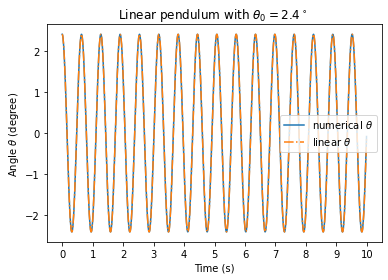
\includegraphics[width=0.6\textwidth]{images/linear_theta.png}
			\caption{Comparison between the analytical and numerical solutions for the linear pendulum.}
			\label{fig:linear_theta}
		\end{figure}
	\end{tcolorbox}

	\newpage
	\item 
	Let's consider a nonlinear pendulum, i.e., $\sin \theta = \theta$, which is released from a standstill at $\theta=\ang{124}$. What is the total energy if you solve the motion equation exactly without any numerical errors? Use the velocity Verlet method to solve it numerically. Plot the energy as a function of time and show at least 12 swing periods. Compare the exact and numerical energies. Generally increase your time step until you find an obvious energy drift; that is, the total energy increases or decreases over a long time (not short time fluctuations). See, e.g., \url{https://en. wikipedia.org/wiki/Energy_drift}. Discuss your findings.
	\begin{tcolorbox}[breakable]
		Assuming $m = \SI{1}{kg}$, the total energy of the system is given by:
		\begin{equation}
			E = K_{max} = U_{max} = m g l (1-\cos{\theta_0}) = \SI{1.528}{J}
		\end{equation}
		We choose this value because the potential energy of the system is zero when the kinetic energy is maximum. 

		The error analysis of the energy $\Delta E$ is given by:
		\begin{align*}
			\Delta E 
			& = \frac{1}{2} m l^2 \Delta(\omega^2) - m g l \Delta(1-\cos{\theta}) \\
			& = \frac{1}{2} m l^2 \Delta(\omega^2) - m g l \Delta(\theta^2 + \dots) \\
			& = \mathcal{O}((1 + \mathcal{O}(h^2))^2) + \mathcal{O}((1 + \mathcal{O}(h^4))^2) \\
			& = \mathcal{O}(h^2) 
		\end{align*}

		The source code for the numerical simulation for the nonlinear pendulum is given in Appendix \ref{nonlinear_py}. Comparison of the numerical solution of the nonlinear pendulum angle using velocity verlet method and linear approximation is given in Figure \ref{fig:nonlinear_theta}. It verifies that the linear approximation is not a good approximation when the angular amplitude is large. 

		\begin{figure}[H]
			\centering
			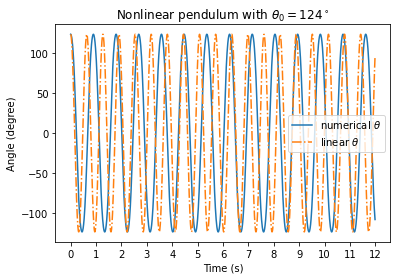
\includegraphics[width=0.6\textwidth]{images/nonlinear_theta.png}
			\caption{Linear approximation vs and numerical solutions for nonlinear pendulum.}
			\label{fig:nonlinear_theta}	
		\end{figure}

		The total energy of the system is given in Figure \ref{fig:nonlinear_energy}. It shows that when using $h = \SI{0.01}{s}$, the standard deviation of the energy is $\SI{0.00098}{J}$, which is much smaller than the total energy. Thus, the energy drift is negligible. 

		\begin{figure}[H]
			\centering
			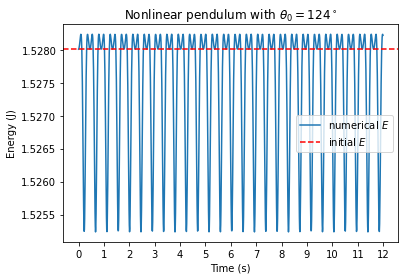
\includegraphics[width=0.6\textwidth]{images/nonlinear_energy.png}
			\caption{Total energy of the nonlinear pendulum as a function of time.}
			\label{fig:nonlinear_energy}
		\end{figure}

		When we use $h = 0.12$, we can see that the energy drift is significant. The standard deviation of the energy is $\SI{0.17}{J}$, which is comparable to the total energy. Figure \ref{fig:nonlinear_drift_theta} and \ref{fig:nonlinear_drift_energy} shows the angle and total energy of the nonlinear pendulum when $h = 0.12$. The energy drift is caused by the numerical error in the velocity Verlet method, which is in order of $\mathcal{O}(h^2)$

		\begin{figure}[H]
			\centering
			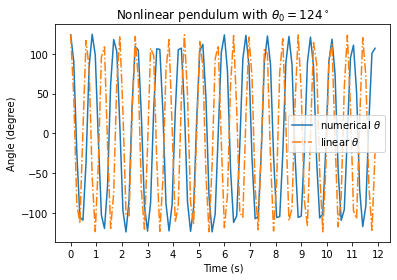
\includegraphics[width=0.6\textwidth]{images/nonlinear_drift_theta.png}
			\caption{Angle of the nonlinear pendulum when $h = 0.12$.}
			\label{fig:nonlinear_drift_theta}
		\end{figure}

		\begin{figure}[H]
			\centering
			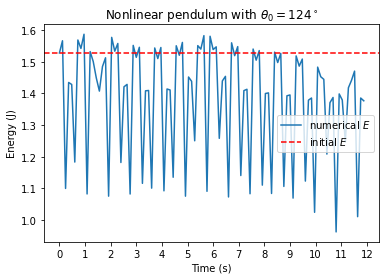
\includegraphics[width=0.6\textwidth]{images/nonlinear_drift_energy.png}
			\caption{Total energy of the nonlinear pendulum when $h = 0.12$.}
			\label{fig:nonlinear_drift_energy}
		\end{figure}

		For longer simulation time, we can see both angle and energy further drifts. Figure \ref{fig:nonlinear_drift_theta_energy2} shows the angle and total energy of the nonlinear pendulum when $h = 0.12$ and $t = \SI{30}{s}$.

		\begin{figure}[H]
			\centering
			\begin{minipage}{0.45\textwidth}
				\centering
				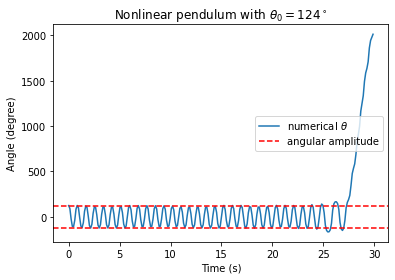
\includegraphics[width=\linewidth]{images/nonlinear_drift_theta2.png}
			\end{minipage}
			\begin{minipage}{0.45\textwidth}
				\centering
				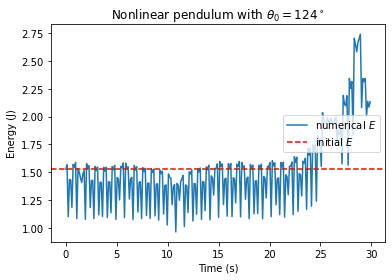
\includegraphics[width=\linewidth]{images/nonlinear_drift_energy2.png}
			\end{minipage}
			\caption{Angle and energy of the nonlinear pendulum for $h = 0.12$ and $t = \SI{30}{s}$.}
			\label{fig:nonlinear_drift_theta_energy2}
		\end{figure}
	\end{tcolorbox}
\end{enumerate}
\end{section}

\newpage
\begin{section*}{Appendix}
	\begin{enumerate}[1.]
		\item \label{linear_py} Linear pendulum numerical simulation ($\theta_0 = 2.4^\circ$)
		\begin{minted}[mathescape,
		linenos,
		numbersep=5pt,
		gobble=2,
		frame=lines,
		framesep=2mm]{python}
		x_init = 2.4*pi/180     # initial angle
		v_init = 0              # initial angular velocity
		t_init = 0
		t_final = 10
		h = 0.01                # time step in second
		
		m = 1
		g = 9.8
		l = 10 * 0.01
		I = m*l**2
		
		X, V, T = [], [], []    
		x_curr, v_curr, t_curr = x_init, v_init, t_init # initialize iterator
		
		def calc_tau(x_curr):
			return -m*g*l*sin(x_curr)
		
		for i in range(floor((t_final-t_init)/h)):
			X.append(x_curr)
			V.append(v_curr)
			T.append(t_curr)
			tau_curr = calc_tau(x_curr)
			x_next = x_curr + h*v_curr + tau_curr/(2*I)*h**2
			tau_next = calc_tau(x_next)
			v_next = v_curr + (tau_curr+tau_next)/(2*I)*h
			t_next = t_curr + h
			x_curr, v_curr, t_curr = x_next, v_next, t_next
		
		X_linear = x_init*np.cos(sqrt(g/l)*np.array(T))
		
		plt.plot(T, np.array(X)*180/pi, label=r"numerical $\theta$")
		plt.plot(T, np.array(X_linear)*180/pi, '-.', label=r"linear $\theta$")
		plt.xlabel("Time (s)")
		plt.ylabel(r"Angle $\theta$ (degree)")
		plt.legend(loc="center right")
		plt.title(r"Linear pendulum with $\theta_0 = 2.4^\circ$ ")
		plt.xticks(np.arange(0, t_final+1, 1))
		plt.show()
		\end{minted}

		\newpage
		\item \label{nonlinear_py} Nonlinear pendulum numerical simulation ($\theta_0 = 124^\circ$)
		\begin{minted}[mathescape,
		linenos,
		numbersep=5pt,
		gobble=2,
		frame=lines,
		framesep=2mm]{python}
		x_init = 124*pi/180     # initial angle
		v_init = 0              # initial angular velocity
		t_init = 0
		t_final = 12
		
		h = 0.01                # time step in second
		# h = 0.12                # toggle this line to see the energy drift
		
		m = 1
		g = 9.8
		l = 10 * 0.01
		I = m*l**2
		
		X, V, T = [], [], []    
		x_curr, v_curr, t_curr = x_init, v_init, t_init # initialize iterator
		
		def calc_tau(x_curr):
			return -m*g*l*sin(x_curr)
		
		for i in range(floor((t_final-t_init)/h)):
			X.append(x_curr)
			V.append(v_curr)
			T.append(t_curr)
			tau_curr = calc_tau(x_curr)
			x_next = x_curr + h*v_curr + tau_curr/(2*I)*h**2
			tau_next = calc_tau(x_next)
			v_next = v_curr + (tau_curr+tau_next)/(2*I)*h
			t_next = t_curr + h
			x_curr, v_curr, t_curr = x_next, v_next, t_next
		
		X_linear = x_init*np.cos(sqrt(g/l)*np.array(T))
		
		plt.plot(T, np.array(X)*180/pi, label=r"numerical $\theta$")
		plt.plot(T, np.array(X_linear)*180/pi, '-.', label=r"linear $\theta$")
		# plt.axhline(y=x_init*180/pi, color='r', linestyle='--', label=r"angular amplitude")
		# plt.axhline(y=-x_init*180/pi, color='r', linestyle='--',)
		plt.title(r"Nonlinear pendulum with $\theta_0 = 124^\circ$")
		plt.xlabel(r"Time (s)")
		plt.ylabel(r"Angle (degree)")
		plt.legend(loc="center right")
		plt.xticks(np.arange(0, t_final+1, 1))
		plt.show()
		
		E = m*g*l*(1-np.cos(np.array(X))) + 1/2*m*l**2*np.array(V)**2
		
		plt.plot(T, E, label=r"numerical $E$")
		plt.axhline(y=m*g*l*(1-cos(x_init)), color='r', linestyle='--', label=r"initial $E$")
		plt.title(r"Nonlinear pendulum with $\theta_0 = 124^\circ$")
		plt.legend(loc="center right")
		plt.xlabel(r"Time (s)")
		plt.ylabel(r"Energy (J)")
		plt.xticks(np.arange(0, t_final+1, 1))
		# plt.ylim(0, max(E))
		plt.show()
		
		print(f"initial energy $E$ = {m*g*l*(1-cos(x_init)):.3f} J")
		print(f"standard deviation of $E$ = {np.std(E)}")
		\end{minted}

	\end{enumerate}
\end{section*}
\end{document}
